\documentclass{report}
\usepackage{fancyhdr} % Required for custom headers
\usepackage{lastpage} % Required to determine the last page for the footer
\usepackage{extramarks} % Required for headers and footers
\usepackage{graphicx} % Required to insert images

\usepackage{amsmath}
\usepackage{graphicx} 
\usepackage{float}
%\usepackage{amsfont}
%\usepackage{amssymb}

\usepackage{multicol}
% Margins
\topmargin=-0.5in
\evensidemargin=0in
\oddsidemargin=-0.5in
\textwidth=7.5in
\textheight=9.0in
\headsep=0.25in 


\pagestyle{fancy}

%\rhead{\textbf{Marshall's Recipes}} % Top right header
%\lhead{\textbf{Curry Stir Fry}}
%\chead{ }
%\title{Curry Stir Fry}

\begin{document}
%\vspace{8mm}
%\textbf{PRELIMINARIES:}


\bigskip

\bigskip

\begin{multicols}{2}
\textbf{Ingredients}
\begin{itemize}
\item 1 lb white mushrooms \newline (130 kCal / 13 gP / 0 gF / 13 gC)
\item $1\frac{1}{2}$ cups arborio rice \quad (1,074 kCal / 20 gP / 2 gF / 237 gC)
\item 10 oz. grape tomatoes  \quad (47 kCal / 2 gP / 0 gF / 10 gC)
\item 1 yellow onion (45 kCal / 1 gP / 0 gF / 11 gC)
\item $\frac{1}{2}$ cup parmesan cheese \newline (216 kCal / 19 gP / 15 gF / 2 gC)
\item 1 tbsp. olive oil \newline (119 kCal / 0 gP / 14 gF / 0 gC)
\item 2 tbsp. butter \quad (204 kCal / 0 gP / 24 gF / 0 gC)
\item 4 cups vegetable or chicken broth (1 box)

\item 5 cloves of garlic
\item Salt to taste
\item $2$ tsp. dried thyme
\item 1 tsp. rosemary
\item green onions (optional garnish)




\end{itemize}


\columnbreak
\textbf{Procedure:}
\medskip


\begin{enumerate}

\item Wash and slice the mushrooms. Put on medium-high heat in a large pan with a pinch of salt. Cook until mushrooms are brown and they release the water, then reduce to medium heat and let the water boil off. 
\item Add one box of chicken stock to a medium saucepan and bring to a boil. Once boiling, reduce to a simmer. 
\item While the mushrooms cook, dice an onion. When mushrooms are finished, remove and set aside. Add the onion to the pan with a tablespoon of olive oil and cook until slightly softened. 
\item When the onions are softened, add garlic, rice, and 1 tbsp. butter. Cook on medium heat for a couple of minutes, until garlic is fragrant. 
\item Adding about $\frac{1}{2}$ cup at a time, add chicken stock into the rice. When the rice has absorbed the stock, add more. Repeat until about $\frac{1}{4}$ of the chicken stock remains. 
\item Slice the grape tomatoes in half and add to pan and continue adding chicken stock.

\item When the rice has fully absorbed all of the chicken stock (approx. 30 minutes), add mushrooms back in, along with 1 tbsp butter, and stir in about $\frac{1}{2}$ cup of parmesan cheese. Once the cheese melts and everything is combined, remove from heat. 
\item Season with salt, rosemary, and thyme to taste. Garnish with chopped green onions on top, if desired. 


\begin{table}[H]
  \begin{center}
    \caption{Macro totals}
    \label{tab:table1}
    \begin{tabular}{c|c|c|c} % <-- Alignments: 1st column left, 2nd middle and 3rd right, with vertical lines in between
      \textbf{Calories} & \textbf{Protein} & \textbf{Fat} & \textbf{Carbs}\\
      \hline
      1,835 kCal & 54 g & 55 g & 273 g\\
    \end{tabular}
  \end{center}
\end{table}
 
\end{enumerate}
\end{multicols}




%\begin{center}
%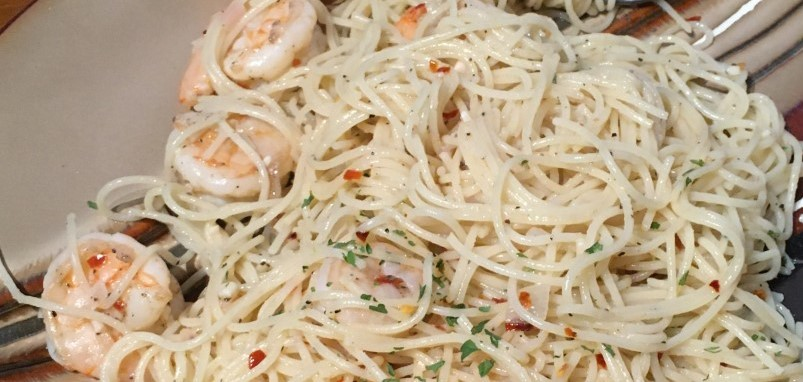
\includegraphics[scale=0.65]{Pasta/Shrimp Scampi/Shrimp Scampi.jpg}
%\end{center}


\end{document}